\begin{problem}{Супчик}{стандартный ввод}{стандартный вывод}{1 секунда}{256 мегабайт}

\begin{figure}[h]
\center{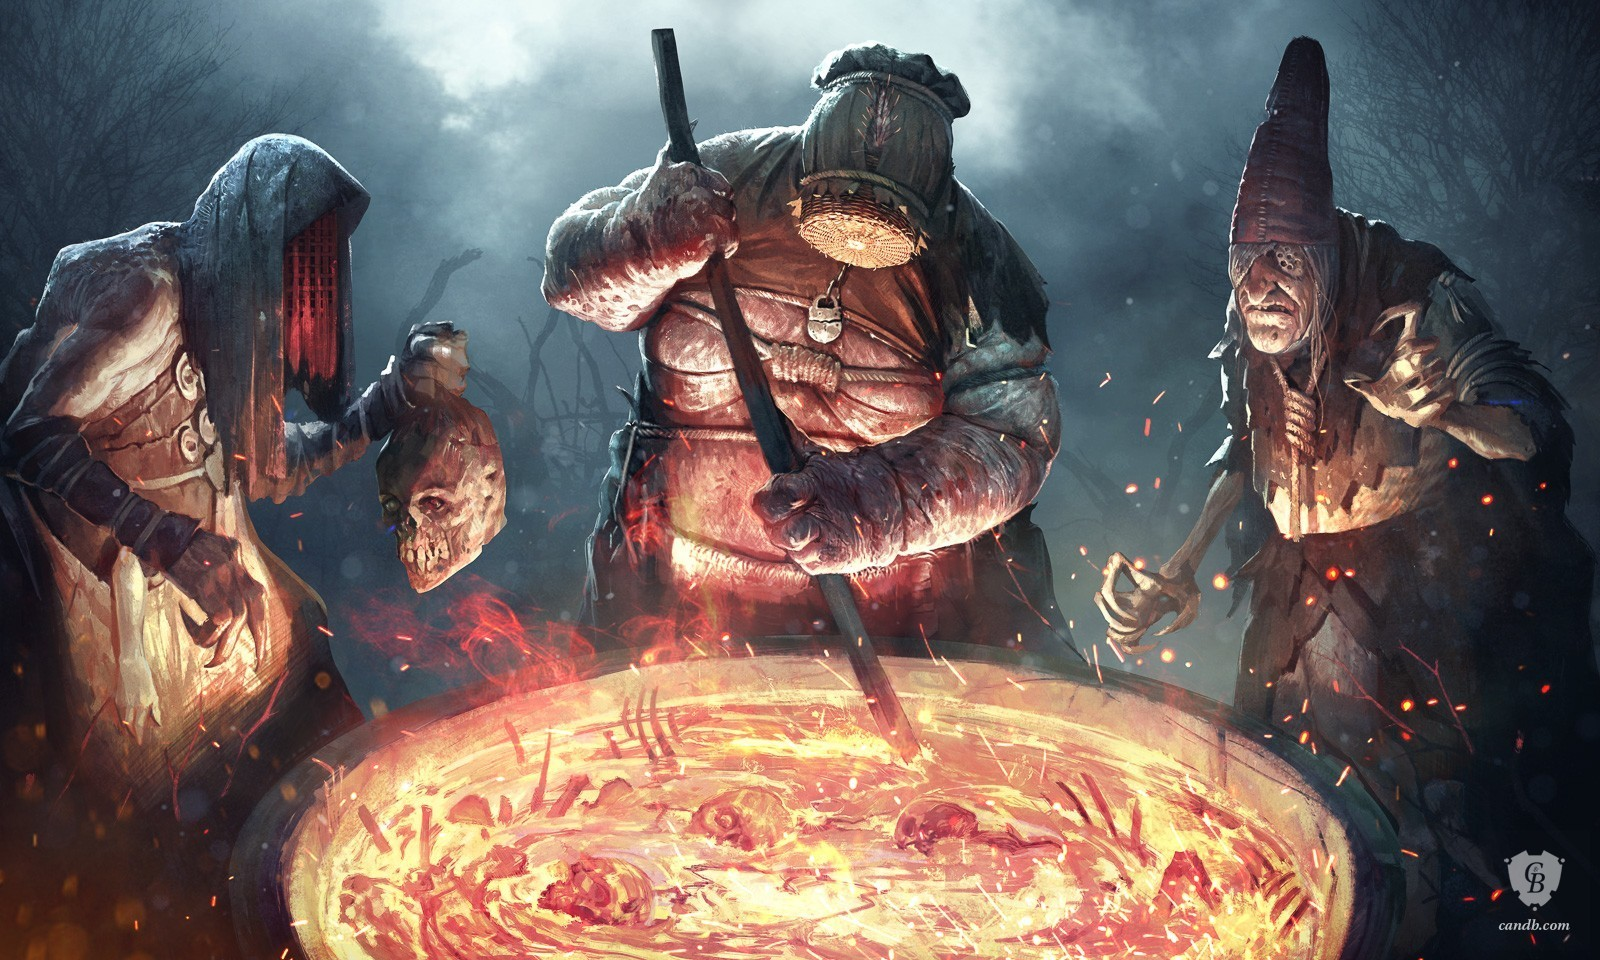
\includegraphics[width=0.6\linewidth,natwidth=1600,natheight=960]{A.jpg} \\}
\end{figure}

Три ведьмы~---~Пряха, Кухарка и Шептуха каждое полнолуние варият себе омолаживающий супчик. Такой особый суп может быть приготовлен только из особых компонентов, а именно костей младенцев, 
крови единорога и истинно любящего сердца. В своей пещере на Кривоуховом болоте у самой дальней стены стоит огромный стеллаж, в каждом ящичке которого лежат неповторимые ингридиенты.
Для того, чтобы не запутаться Шептуха присвоила каждому ящику свой индивидуальный номер~---~так костям младенцев соответсвует номер 4, любящему сердцу номер 13, а самому редкому компоненту~---~крови единорога~---~666. 
Именно в день полной луны она решила пойти в деревню за новой порцией свежих детей, поэтому
она оставила своим сестрам записку, где указала номера нужных ингридиентов. Сестры уже плохо видят в связи с довольно почтенным возрастом и из-за этого могли пару раз ошибиться.
По возвращению Шептуха решила проверить состав их варева. Помогите ей сделать это.


\InputFile
На вход подаются натуральные числа $N, M (0 < N, M < 100)$~---~размер котла. Затем двумерный массив, описывающий ингридиенты, плавающие в супчике, состоящий из натуральных чисел - номеров ингридиентов.
Известно, что самый верхний правый ящик имеет номер 1000.

\OutputFile
Вывести \t{YES}, если все элементы супа собраны правильно, и \t{NO}~---~если нет.

\Example

\begin{example}
\exmp{3 3
4 111 56
999 45 15
13 55 666
}{NO
}%
\end{example}

\end{problem}

